% !Rnw weave = knitr
% =============================================================
% Proyecto: Accidentes gestionados por la Guardia Urbana de Barcelona
% Reto 2 - Punto 5: informe técnico con knitr
%
% Este documento está escrito en formato .Rnw: combina codigo LaTeX
% con bloques de codigo R (chunks) que se ejecutan al compilar.
% Los resultados númericos del texto no están escritos a mano, se
% insertan mediante \Sexpr{}, de modo que se recalculan solos si
% cambian los datos de origen. 
%
% PARA COMPILAR: abrir en RStudio y pulsar "Compile PDF".
% Requiere una distribucion de LaTeX (tinytex).
% =============================================================

\documentclass[11pt,a4paper]{article}\usepackage[]{graphicx}\usepackage[]{xcolor}
% maxwidth is the original width if it is less than linewidth
% otherwise use linewidth (to make sure the graphics do not exceed the margin)
\makeatletter
\def\maxwidth{ %
  \ifdim\Gin@nat@width>\linewidth
    \linewidth
  \else
    \Gin@nat@width
  \fi
}
\makeatother

\definecolor{fgcolor}{rgb}{0.345, 0.345, 0.345}
\newcommand{\hlnum}[1]{\textcolor[rgb]{0.686,0.059,0.569}{#1}}%
\newcommand{\hlsng}[1]{\textcolor[rgb]{0.192,0.494,0.8}{#1}}%
\newcommand{\hlcom}[1]{\textcolor[rgb]{0.678,0.584,0.686}{\textit{#1}}}%
\newcommand{\hlopt}[1]{\textcolor[rgb]{0,0,0}{#1}}%
\newcommand{\hldef}[1]{\textcolor[rgb]{0.345,0.345,0.345}{#1}}%
\newcommand{\hlkwa}[1]{\textcolor[rgb]{0.161,0.373,0.58}{\textbf{#1}}}%
\newcommand{\hlkwb}[1]{\textcolor[rgb]{0.69,0.353,0.396}{#1}}%
\newcommand{\hlkwc}[1]{\textcolor[rgb]{0.333,0.667,0.333}{#1}}%
\newcommand{\hlkwd}[1]{\textcolor[rgb]{0.737,0.353,0.396}{\textbf{#1}}}%
\let\hlipl\hlkwb

\usepackage{framed}
\makeatletter
\newenvironment{kframe}{%
 \def\at@end@of@kframe{}%
 \ifinner\ifhmode%
  \def\at@end@of@kframe{\end{minipage}}%
  \begin{minipage}{\columnwidth}%
 \fi\fi%
 \def\FrameCommand##1{\hskip\@totalleftmargin \hskip-\fboxsep
 \colorbox{shadecolor}{##1}\hskip-\fboxsep
     % There is no \\@totalrightmargin, so:
     \hskip-\linewidth \hskip-\@totalleftmargin \hskip\columnwidth}%
 \MakeFramed {\advance\hsize-\width
   \@totalleftmargin\z@ \linewidth\hsize
   \@setminipage}}%
 {\par\unskip\endMakeFramed%
 \at@end@of@kframe}
\makeatother

\definecolor{shadecolor}{rgb}{.97, .97, .97}
\definecolor{messagecolor}{rgb}{0, 0, 0}
\definecolor{warningcolor}{rgb}{1, 0, 1}
\definecolor{errorcolor}{rgb}{1, 0, 0}
\newenvironment{knitrout}{}{} % an empty environment to be redefined in TeX

\usepackage{alltt}

\usepackage[utf8]{inputenc}
\usepackage[T1]{fontenc}
\usepackage[spanish,es-tabla,es-noquoting]{babel}
\usepackage{graphicx}
\usepackage{booktabs}
\usepackage{float}
\usepackage[margin=2.5cm]{geometry}
\usepackage{hyperref}
\hypersetup{colorlinks=true, linkcolor=black, urlcolor=blue}

\title{Siniestralidad vial en Barcelona, 2019--2025\\
       \large Informe técnico}
\author{Ioana Bendris Greab}
\date{\today}
\IfFileExists{upquote.sty}{\usepackage{upquote}}{}
\begin{document}

\maketitle



\begin{abstract}
\noindent
Este informe analiza los 54.954 accidentes de tráfico
gestionados por la Guàrdia Urbana de Barcelona entre 2019 y 2025. El
resultado principal es que la reducción del número de siniestros no se ha
traducido en una reducción equivalente de su gravedad: mientras el volumen
de accidentes descendió un 22.8\,\%, la
proporción de siniestros graves o mortales pasó del
2.06\,\% al 3.26\,\%. El
análisis territorial muestra además que volumen y riesgo son dimensiones
independientes, con una correlación de apenas
0.1 entre ambas.
\end{abstract}

\tableofcontents
\newpage

% =============================================================
\section{Introducción y objetivos}
% =============================================================

La seguridad viaria constituye una de las competencias municipales con
mayor impacto directo sobre la salud pública. Barcelona publica desde hace
años los accidentes gestionados por su policía local, lo que permite
analizar la evolución de la siniestralidad con un nivel de detalle
territorial y temporal poco habitual.

\subsection{Objetivo principal}

Analizar la evolución y la distribución de la siniestralidad vial en
Barcelona entre 2019 y 2025, con el fin de determinar en qué medida la
reducción del número de accidentes se ha acompañado de una reducción
equivalente de su gravedad, y qué zonas y momentos concentran el riesgo
más alto.

\subsection{Objetivos específicos}

\begin{enumerate}
  \item Describir la evolución temporal del número de accidentes y de su
        gravedad, distinguiendo el efecto de la pandemia de la tendencia
        de fondo posterior.
  \item Comparar la siniestralidad entre los diez distritos, en volumen
        absoluto y en proporción de accidentes graves.
  \item Caracterizar los patrones temporales intrasemanales.
  \item Localizar geográficamente los puntos de mayor acumulación de
        accidentes graves.
  \item Evaluar la calidad y las limitaciones del conjunto de datos.
\end{enumerate}

% =============================================================
\section{Datos y método}
% =============================================================

Los datos proceden del conjunto \textit{Accidents gestionats per la
Guàrdia Urbana a la ciutat de Barcelona}, publicado por el Ajuntament de
Barcelona en el portal Open Data BCN bajo licencia Creative Commons
Attribution 4.0. Se han utilizado los siete ficheros anuales del periodo
2019--2025, que suman 54.954 registros.

\subsection{Depuración}

La unificación de los ficheros anuales requirió resolver siete
incidencias de homogeneidad. La más relevante afecta a la comparabilidad
de la serie: \textbf{en 2024 y 2025 los valores cero se registran como
celda vacía}, mientras que en los años anteriores se escribe un cero
explícito. Interpretar esos blancos como dato desconocido habría supuesto
descartar el 97\,\% de los accidentes recientes al clasificar la gravedad.
La imputación como cero se validó comprobando la coherencia del resultado
con la serie histórica de la ciudad.

Otras incidencias resueltas: cambios en los nombres de columna entre años,
columnas presentes solo en algunos ficheros, el valor $-1$ como código de
dato no disponible, el campo \texttt{Codi\_barri} con formato incompatible
en 2020, la inferencia automática de tipos que corrompía el identificador
de expediente, y espacios sobrantes en los campos de texto.

\subsection{Definición de gravedad}

Los datos originales reparten la severidad en tres columnas de recuento
independientes. Se derivó una variable ordinal de tres
niveles: un accidente es \textit{mortal} si registra alguna persona
fallecida, \textit{grave} si registra alguna herida grave sin fallecidos,
y \textit{leve} en el resto de casos.

% =============================================================
\section{Resultados}
% =============================================================

\subsection{Panorama general}

En el conjunto del periodo se registraron 54.954 accidentes,
que causaron 61.474 personas heridas leves,
1.418 heridas graves y 115 fallecidas. El
90.3\,\% de los siniestros registrados tuvo al
menos una víctima, lo que indica que el conjunto recoge fundamentalmente
accidentes con daños personales y no incidentes con daños materiales
únicamente.

\begin{table}

\caption{\label{tab:tabla-anual}Indicadores anuales de siniestralidad, 2019--2025}
\centering
\begin{tabular}[t]{rrrrrr}
\toprule
Año & Accidentes & H. leves & H. graves & Fallecidos & \% grave/mortal\\
\midrule
2.019 & 10.027 & 11.640 & 202 & 22 & 2.06\\
2.020 & 6.268 & 7.074 & 142 & 14 & 2.23\\
2.021 & 7.659 & 8.693 & 167 & 12 & 2.14\\
2.022 & 7.999 & 8.893 & 176 & 24 & 2.41\\
2.023 & 7.724 & 8.552 & 228 & 21 & 3.02\\
2.024 & 7.536 & 8.246 & 254 & 11 & 3.30\\
2.025 & 7.741 & 8.376 & 249 & 11 & 3.26\\
\bottomrule
\end{tabular}
\end{table}



\subsection{Evolución temporal (objetivo 1)}

El año 2020 marca una discontinuidad evidente: los accidentes cayeron un
37.5\,\% respecto a 2019 como consecuencia
de las restricciones de movilidad. Lo relevante es que \textbf{el nivel
prepandemia no se ha recuperado}: en 2025 se registraron
7.741 accidentes, frente a los 10.027 de
2019.

\begin{knitrout}
\definecolor{shadecolor}{rgb}{0.969, 0.969, 0.969}\color{fgcolor}\begin{figure}[H]

{\centering 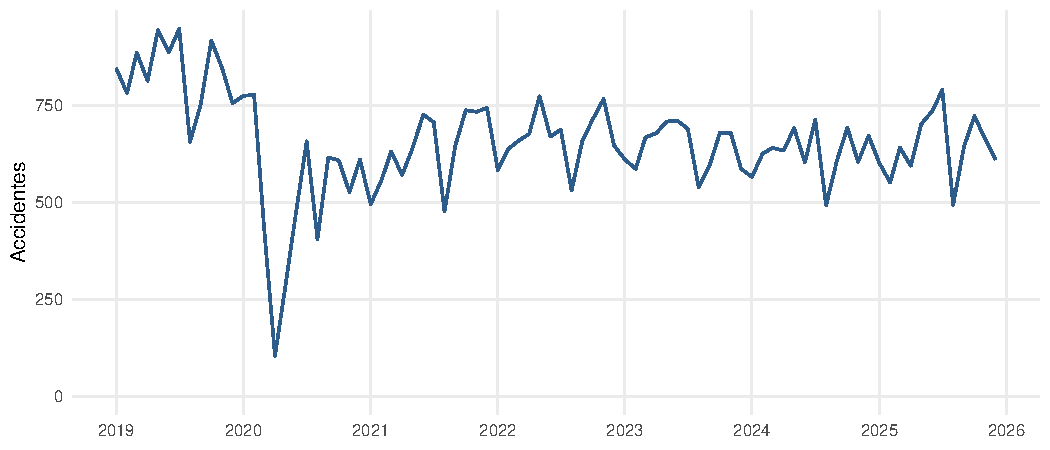
\includegraphics[width=0.85\textwidth]{figuras/fig-evolucion-1} 

}

\caption[Evolución mensual del número de accidentes]{Evolución mensual del número de accidentes}\label{fig:fig-evolucion}
\end{figure}

\end{knitrout}

Sin embargo, la reducción del volumen no ha ido acompañada de una
reducción proporcional de la gravedad. La figura~\ref{fig:fig-gravedad}
contrapone ambas magnitudes: los accidentes graves aumentaron de
185 en 2019 a 241 en 2025, pese a
producirse casi un tercio menos de siniestros. Los fallecidos, en cambio,
descendieron de 22 a 11.

\begin{knitrout}
\definecolor{shadecolor}{rgb}{0.969, 0.969, 0.969}\color{fgcolor}\begin{figure}[H]

{\centering 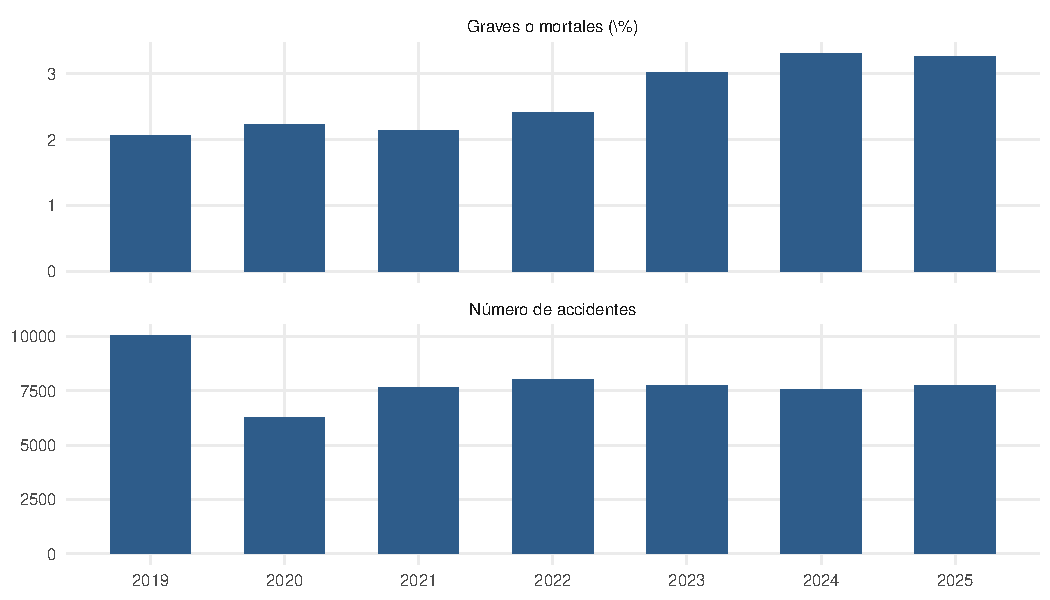
\includegraphics[width=0.85\textwidth]{figuras/fig-gravedad-1} 

}

\caption[Volumen de accidentes frente a proporción de siniestros graves o mortales]{Volumen de accidentes frente a proporción de siniestros graves o mortales}\label{fig:fig-gravedad}
\end{figure}

\end{knitrout}

Este resultado admite varias interpretaciones que los datos disponibles no
permiten discriminar. Una hipótesis plausible es un cambio en la
composición del parque circulante, con mayor presencia de motocicletas y
vehículos de movilidad personal, cuyos usuarios están más expuestos en
caso de colisión. Verificar esta hipotesis supondría tener datos sobre el
tipo de vehículo implicado, datos ausentes en este conjunto.

\subsection{Distribución territorial (objetivo 2)}

El distrito con más accidentes es Eixample,
con 15.080 siniestros, más de una cuarta
parte del total de la ciudad. Su gravedad relativa, sin embargo, es
2.59\,\%, próxima a la media municipal de
2.62\,\%.

El distrito con mayor gravedad relativa es
Horta-Guinardó
(3.41\,\%), y el de menor
Sant Andreu
(1.96\,\%).

\begin{knitrout}
\definecolor{shadecolor}{rgb}{0.969, 0.969, 0.969}\color{fgcolor}\begin{figure}[H]

{\centering 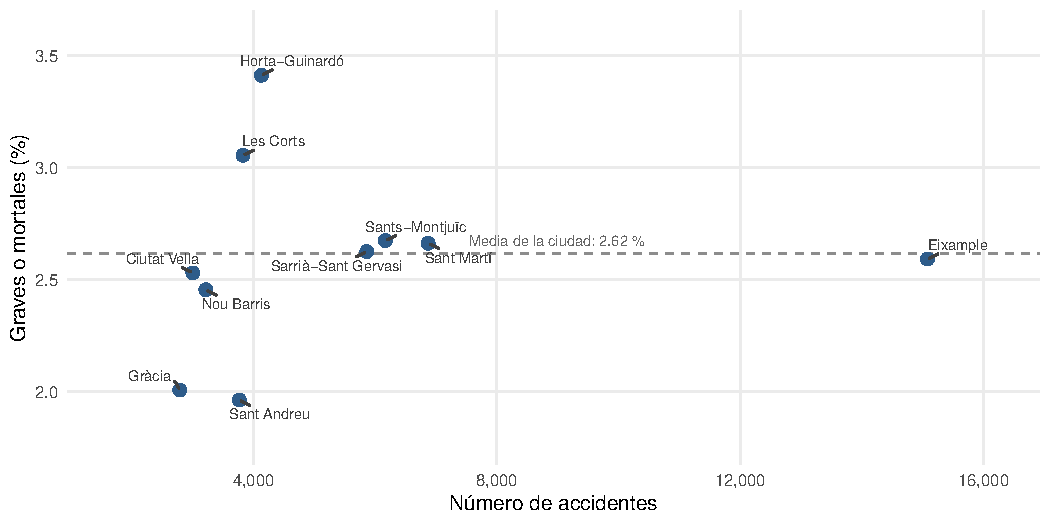
\includegraphics[width=0.85\textwidth]{figuras/fig-distritos-1} 

}

\caption[Relación entre volumen de accidentes y gravedad relativa por distrito]{Relación entre volumen de accidentes y gravedad relativa por distrito}\label{fig:fig-distritos}
\end{figure}

\end{knitrout}

La correlación de Pearson entre ambas magnitudes es de
0.1, prácticamente nula. \textbf{Volumen y
riesgo son, por tanto, dimensiones independientes.} La implicación
práctica es directa: priorizar las actuaciones únicamente en función del
número de accidentes dejaría sin atender los distritos donde el riesgo por
siniestro es mayor.

Conviene subrayar que esta comparación no equivale a un ranking de
peligrosidad. Sin datos sobre la intensidad de tráfico soportada por cada
distrito, las cifras reflejan tanto el riesgo como la exposición.

\subsection{Patrones temporales (objetivo 3)}

El día con más accidentes es el viernes
(9.179) y el que menos el
domingo
(4.828). La hora de máxima concentración son las
14~h.

Se repite aquí el patrón inverso observado en el análisis territorial: el
domingo presenta la mayor
proporción de accidentes graves
(3.07\,\%) siendo uno de los días con menos
siniestros. Que dos dimensiones independientes muestren la misma relación
inversa refuerza la interpretación de fondo: menor densidad de tráfico se
asocia a mayor velocidad y, con ella, a consecuencias más severas.

\begin{knitrout}
\definecolor{shadecolor}{rgb}{0.969, 0.969, 0.969}\color{fgcolor}\begin{figure}[H]

{\centering 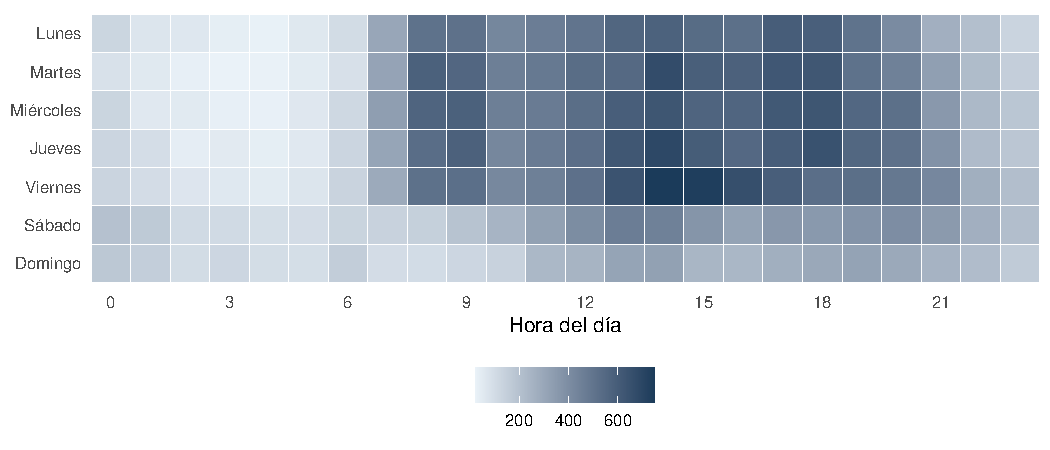
\includegraphics[width=0.85\textwidth]{figuras/fig-heatmap-1} 

}

\caption[Concentración de accidentes por hora y día de la semana]{Concentración de accidentes por hora y día de la semana}\label{fig:fig-heatmap}
\end{figure}

\end{knitrout}

\subsection{Localización del riesgo (objetivo 4)}

\begin{table}

\caption{\label{tab:tabla-vias}Vías con mayor número de accidentes registrados}
\centering
\begin{tabular}[t]{lrr}
\toprule
Vía & Accidentes & Graves o mortales\\
\midrule
Corts Catalanes & 2.328 & 58\\
Diagonal & 1.958 & 65\\
Aragó & 1.364 & 27\\
Meridiana & 924 & 21\\
Dalt (Besòs) & 774 & 18\\
València & 744 & 18\\
Litoral (Llobregat) & 699 & 25\\
Dalt (Llobregat) & 695 & 24\\
\bottomrule
\end{tabular}
\end{table}



Los grandes ejes viarios estructuran la distribución del riesgo. La
concentración en vías de alta capacidad resulta coherente con la
interpretación anterior: son los viales donde se alcanzan velocidades
mayores dentro del entorno urbano.

% =============================================================
\section{Calidad del dato (objetivo 5)}
% =============================================================

El conjunto presenta una cobertura muy alta en las variables esenciales.
Únicamente el
0.42\,\% de los
registros carece de ubicación administrativa y el
0.08\,\% de
coordenadas geográficas válidas.

La principal limitación no es la ausencia de datos, sino la
\textbf{heterogeneidad de los criterios de registro entre años}. Los
cambios documentados en el apartado 2 obligan a interpretar con cautela
cualquier comparación que abarque el periodo completo.

% =============================================================
\section{Conclusiones}
% =============================================================

\begin{enumerate}
  \item La siniestralidad vial en Barcelona ha descendido un
        22.8\,\% entre 2019 y 2025, sin
        recuperar el nivel prepandemia.
  \item Ese descenso no se ha traducido en menos víctimas graves: los
        accidentes graves aumentaron de 185 a
        241. Los fallecidos, en cambio, se redujeron de
        22 a 11.
  \item Volumen y gravedad son dimensiones territorialmente
        independientes (correlación de 0.1), lo
        que desaconseja priorizar actuaciones atendiendo solo al recuento
        de siniestros.
  \item Los momentos de menor tráfico concentran proporcionalmente más
        accidentes graves, patrón que se observa tanto en la dimensión
        semanal como en la territorial.
\end{enumerate}

% =============================================================
\section*{Limitaciones}
\addcontentsline{toc}{section}{Limitaciones}
% =============================================================

El conjunto recoge únicamente los siniestros gestionados por la Guàrdia
Urbana, de modo que no incluye los accidentes no reportados. Al no
disponerse de datos de intensidad de tráfico ni de desplazamientos, no es
posible calcular tasas de riesgo por vehículo-kilómetro: todas las cifras
se refieren a accidentes registrados, no a riesgo por desplazamiento. Por
último, la ausencia de información sobre el tipo de vehículo implicado
impide contrastar la hipótesis más plausible sobre el aumento de la
gravedad.

% =============================================================
\section*{Reproducibilidad}
\addcontentsline{toc}{section}{Reproducibilidad}
% =============================================================

Este documento se ha generado con \texttt{knitr}. Todas las cifras que
aparecen en el texto se calculan al compilar mediante \verb|\Sexpr{}|, y
todos los gráficos y tablas se producen a partir de los datos depurados en
el momento de la compilación. 

El código de depuración, el dashboard y este informe están disponibles en
el repositorio del proyecto.

\begin{knitrout}
\definecolor{shadecolor}{rgb}{0.969, 0.969, 0.969}\color{fgcolor}\begin{kframe}
\begin{alltt}
\hlcom{# La información de sesion documenta las versiones exactas de R y de}
\hlcom{# los paquetes utilizados, requisito habitual en investigacion}
\hlcom{# reproducible para que un tercero pueda replicar el entorno.}
\hlkwd{sessionInfo}\hldef{()}\hlopt{$}\hldef{R.version}\hlopt{$}\hldef{version.string}
\end{alltt}
\begin{verbatim}
[1] "R version 4.5.2 (2025-10-31)"
\end{verbatim}
\end{kframe}
\end{knitrout}

\end{document}
